\PassOptionsToPackage{subsection=false}{beamerouterthememiniframes} %removes the subsection bar in each frame
\documentclass[hyperref={pdfpagelabels=false},unknownkeysallowed]{beamer}
\mode<presentation>
\usetheme{Szeged} %\usetheme{Berkeley} \usecolortheme{seagull} \setbeamercolor{structure}{bg=green!40!gray!50!white} \setbeamercolor{palette primary}{fg=yellow,bg=yellow} % changed this
\setbeamercolor{background canvas}{bg=white!90!gray}%parent=normal text}
%\usecolortheme{seahorse}
%\usecolortheme{sidebartab}
\setbeamercolor{itemize item}{fg=green!80!black}
\setbeamercolor{enumerate item}{fg=gray}
\setbeamercolor{frametitle}{fg=red!40!blue!50!black,bg=gray!40}
\setbeamercolor{title}{fg=red!40!blue!50!black,bg=gray!40}

% By  using hyperref={pdfpagelabels=false} you get rid off:
% Package hyperref Warning: Option `pdfpagelabels' is turned off
% (hyperref)                because \thepage is undefined. 
% Hyperref stopped early 
%
\colorlet{titlecolor}{red!40!blue!50!black}
\colorlet{themecolor}{red!40!blue!50!white}
\colorlet{urlcolor}{red!20!blue!70!gray}
\colorlet{filecolor}{red!30!blue!60!black}

\hypersetup{colorlinks=true,linkcolor=darkgray,urlcolor=urlcolor,filecolor=filecolor}


\usepackage{etoolbox}
\usepackage{xcolor}
% this is to include motion pictures
\usepackage{multimedia}
\usepackage{graphicx}
\usepackage{tikz}
\usepackage{pifont}
%%%%%%%%%%%%%%%%
 % define block of various length
     \newenvironment<>{varblock}[2][.9\textwidth]{%
      \setlength{\textwidth}{#1}
      \begin{actionenv}#3%
        \def\insertblocktitle{#2}%
        \par%
        \usebeamertemplate{block begin}}
      {\par%
        \usebeamertemplate{block end}%
      \end{actionenv}}   
%%%%%%%%%%%%%%%%
 % this is just for the progress bar
    \usetikzlibrary{calc}
    \definecolor{pbgray}{HTML}{575757}% background color for the progress bar
    \makeatletter
    \def\progressbar@progressbar{} % the progress bar
    \newcount\progressbar@tmpcounta% auxiliary counter
    \newcount\progressbar@tmpcountb% auxiliary counter
    \newdimen\progressbar@pbht %progressbar height
    \newdimen\progressbar@pbwd %progressbar width
    \newdimen\progressbar@tmpdim % auxiliary dimension
    \progressbar@pbwd=\linewidth
    \progressbar@pbht=1pt
    % the progress bar
    \def\progressbar@progressbar{%
        \progressbar@tmpcounta=\insertframenumber
        \progressbar@tmpcountb=\inserttotalframenumber
        \progressbar@tmpdim=\progressbar@pbwd
        \multiply\progressbar@tmpdim by \progressbar@tmpcounta
        \divide\progressbar@tmpdim by \progressbar@tmpcountb
      \begin{tikzpicture}[very thin]
        \draw[pbgray!30,line width=\progressbar@pbht]
          (0pt, 0pt) -- ++ (\progressbar@pbwd,0pt);
        \draw[draw=none]  (\progressbar@pbwd,0pt) -- ++ (2pt,0pt);
        \draw[fill=pbgray!30,draw=pbgray] %
           ( $ (\progressbar@tmpdim, \progressbar@pbht) + (0,1.5pt) $ ) -- ++(60:3pt) -- ++(180:3pt) ;
        \node[draw=pbgray!30,text width=3.5em,align=center,inner sep=1pt,
          text=pbgray!70,anchor=east] at (0,0) {\insertframenumber/\inserttotalframenumber};
      \end{tikzpicture}%
    }
    \setbeamertemplate{headline}{}
    \setbeamertemplate{footline}{}
    \addtobeamertemplate{footline}{}
    {%
      \begin{beamercolorbox}[wd=\paperwidth,ht=5ex,center,dp=1ex]{white}%
        \progressbar@progressbar%
      \end{beamercolorbox}%
    }
    \makeatother
%%%%%%%%%

\newcommand{\smiley}{\tikz[baseline=-0.75ex,black]{
    \draw circle (2mm);
\node[fill,circle,inner sep=0.5pt] (left eye) at (135:0.8mm) {};
\node[fill,circle,inner sep=0.5pt] (right eye) at (45:0.8mm) {};
\draw (-145:0.9mm) arc (-120:-60:1.5mm);
    }
}

% custom item elements
\newcommand{\titem}{\item[\color{themecolor}\ding{220}]} 
\newcommand{\grayitem}{\item[\color{gray}\ding{220}]}

% 'fill' slide to but stuff at the buttom
\newcommand{\tobottom}{\vskip0pt plus 1filll}



\makeatletter
\patchcmd{\beamer@sectionintoc}{\vskip1.5em}{\vskip0.5em}{}{}
\makeatother
\usepackage{textpos}
%\usepackage[scaled=.90]{helvet}% Helvetica, served as a model for arial

\usepackage{lmodern}
% Using lmondern and you get rid off this:
% LaTeX Font Warning: Font shape `OT1/cmss/m/n' in size <4> not available
% (Font)              size <5> substituted on input line 22.
% LaTeX Font Warning: Size substitutions with differences
% (Font)              up to 1.0pt have occurred.
%

% If \titel{$B!D(B} \author{$B!D(B} come after \begin{document} 
% you get the following warnig:
% Package hyperref Warning: Option `pdfauthor' has already been used,
% (hyperref) ... 
% So it is here before \begin{document}



\title{\textbf{Web Scraping}}   
%\subtitle{P. Lemey, A. Rambaut, A.J. Drummond, M.A. Suchard} 
\date{\today} 
\author{Antoine \& Jonas}
\institute{ETH - TB}

%\usepackage{beamerthemesplit} % new 
% Alternatively, you can also use the usetheme Warsaw
% \usetheme{Warsaw}





\begin{document}
\begin{frame}[plain]
\titlepage
\end{frame} 


\addtobeamertemplate{frametitle}{}{%
\begin{textblock*}{100mm}(.85\textwidth,-1cm)
%\includegraphics[height=1cm]{fig/Trophallaxis.jpg}
\end{textblock*}}

\section{Introduction}
\begin{frame}
    \begin{center}
        \textbf{\small or}
        \vspace*{1cm}
        \textcolor{titlecolor}{\textbf{\huge\\ How to get data from the web to your PC}}
    \end{center}
\end{frame}
% %%%%%%%%%%%%%%%%%%%%%%%%%%%%%%%%%%%%%%%%%%%%%%%%%%%%%%%%%%
% \begin{frame}
%     \frametitle{\textbf{Overview}} %DONT SHOW SUBSECTIONS!
%     \tableofcontents[hideallsubsections]
% \end{frame}
% %%%%%%%%%%%%%%%%%%%%%%%%%%%%%%%%%%%%%%%%%%%%%%%%%%%%%%%%%%
\begin{frame}
        \makebox[\linewidth]{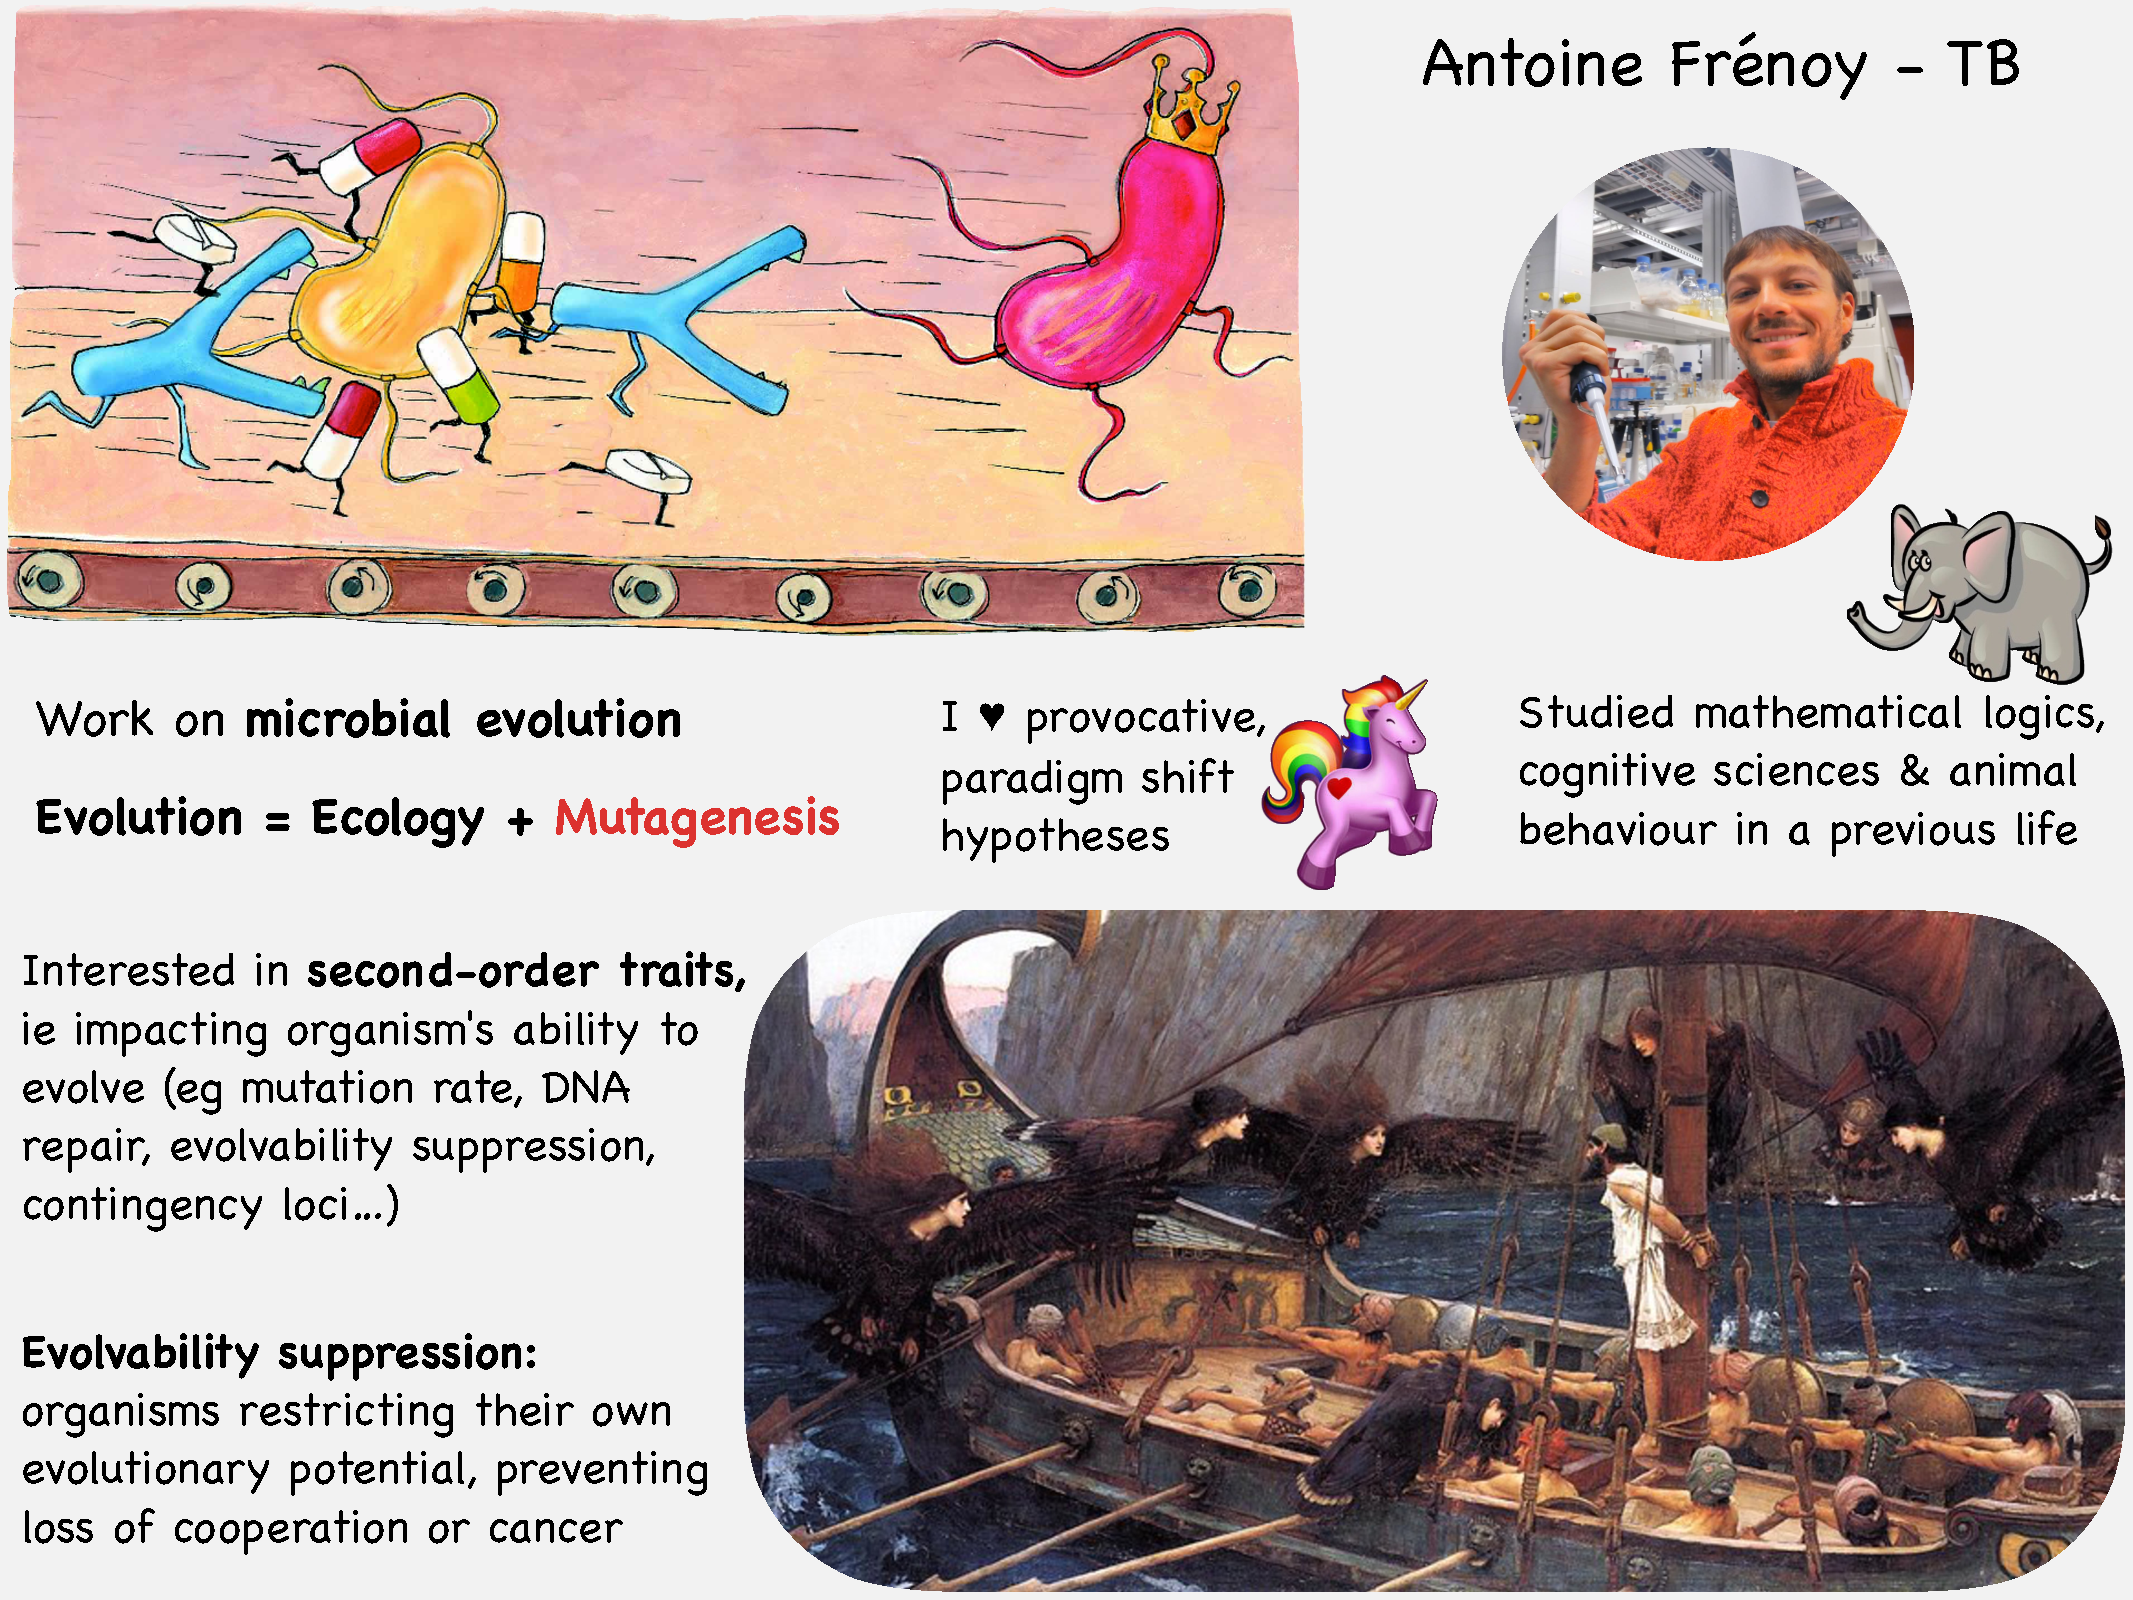
\includegraphics[page=1,width=0.98\paperwidth]{antoine.pdf}}
\end{frame}
\begin{frame}
        \makebox[\linewidth]{\includegraphics[page=2,width=0.98\paperwidth]{antoine.pdf}}
\end{frame}
%%%%%%%%%%%%%%%%%%%%%%%%%%%%%%%%%%%%%%%%%%%%%%%%%%%%%%%%%%
%%%%%%%%%%%%%%%%%%%%%%%%%%%%%%%%%%%%%%%%%%%%%%%%%%%%%%%%%%
\begin{frame}
    \begin{center}
        \textbf{Intro Jonas}
    \end{center}
\end{frame}
%%%%%%%%%%%%%%%%%%%%%%%%%%%%%%%%%%%%%%%%%%%%%%%%%%%%%%%%%%
%%%%%%%%%%%%%%%%%%%%%%%%%%%%%%%%%%%%%%%%%%%%%%%%%%%%%%%%%%
\begin{frame}
    \begin{center}
        \textcolor{titlecolor}{\textbf{\huge\\ How to get data from the web to your PC}}
    \end{center}
\end{frame}
%%%%%%%%%%%%%%%%%%%%%%%%%%%%%%%%%%%%%%%%%%%%%%%%%%%%%%%%%%
\begin{frame}
    \frametitle{\textbf{Overview}}
    \begin{itemize}
        \titem \textbf{Present the \textit{recommended} approach}
        \titem \textbf{Show how to by means of examples}
        \titem \textbf{Provide links for additional reading}
    \end{itemize}
\end{frame}
%%%%%%%%%%%%%%%%%%%%%%%%%%%%%%%%%%%%%%%%%%%%%%%%%%%%%%%%%%
\begin{frame}
    \frametitle{\textbf{Data supply status of server}}
    \begin{itemize}
        \titem \textbf{\textit{The Good}: Provision in raw form}
        \titem \textbf{\textit{The Ugly}: Provision of data representation}
        \titem \textbf{\textit{The Bad}: Data not available}
    \end{itemize}
\end{frame}
%%%%%%%%%%%%%%%%%%%%%%%%%%%%%%%%%%%%%%%%%%%%%%%%%%%%%%%%%%
\begin{frame}
    \frametitle{\textbf{The \textit{Recommended} Approach}}
    \begin{center}
        \begin{enumerate}
            \item \textbf{ Designated provision of raw data:}
                \begin{itemize}
                    \only<1>{\grayitem}\only<2->{\titem} \textbf{Downloadable Content}
                    \only<1>{\grayitem}\only<2->{\titem} \textbf{Application programing interface (API)}
                \end{itemize}
            \item  \textbf{Request raw data}
            \only<1>{\item}\only<2->{\titem} \textbf{Scrape data from HTML}
            % \uncover<2->{
            %     \titem \textbf{What to do with the data afterwards}
            % }
        \end{enumerate}
\vspace*{1cm}
\uncover<2->{
    \textbf{\textcolor{themecolor}{\ding{220}}: What will be covered}
}
    \end{center}
\end{frame}
%%%%%%%%%%%%%%%%%%%%%%%%%%%%%%%%%%%%%%%%%%%%%%%%%%%%%%%%%%
\begin{frame}[label=downloadable_content]
    \frametitle{\textbf{Downloadable Content}}
    \textbf{\Large Server provides a data file}
    \vspace*{0.5cm}
    \begin{itemize}
        \grayitem \textbf{\texttt{Go to the website}, \texttt{click on item}\ldots}
        \titem \textbf{Use the command line, e.g. \hyperlink{commandline}{wget or curl}}
        \titem \textbf{Use web-packages e.g. for python: \hyperlink{commandline}{urllib or requests}}
    \end{itemize}
\end{frame}
%%%%%%%%%%%%%%%%%%%%%%%%%%%%%%%%%%%%%%%%%%%%%%%%%%%%%%%%%%
\begin{frame}[label=api_intro]
    \frametitle{\textbf{API}}
    \textbf{\Large What is an API?}
    \vspace*{0.5cm}
    \begin{itemize}
        \grayitem \textbf{Application Programming Interface}
        \grayitem \textbf{Absence of representational information}
        \grayitem \textbf{Content is assembled \textit{on demand}}
    \end{itemize}
\end{frame}
%%%%%%%%%%%%%%%%%%%%%%%%%%%%%%%%%%%%%%%%%%%%%%%%%%%%%%%%%%
\begin{frame}[label=api_approach]
    \frametitle{\textbf{API}}
    \textbf{\Large How to use an API}
    \vspace*{0.5cm}
    \begin{itemize}
        \grayitem \textbf{If there is an API, there is a Documentation for it}
        \grayitem \textbf{If there is an API, there might be an API for it}
    \end{itemize}
\end{frame}
%%%%%%%%%%%%%%%%%%%%%%%%%%%%%%%%%%%%%%%%%%%%%%%%%%%%%%%%%%
\begin{frame}[label=api_further]
    \frametitle{\textbf{API}}
    \textbf{\Large What is an API?}
    \vspace*{0.5cm}
    \begin{itemize}
        \grayitem \textbf{Application Programming Interface}
        \grayitem \textbf{Absence of representational information}
        \grayitem \textbf{Content is assembled \textit{on demand}}
    \end{itemize}
\end{frame}
%%%%%%%%%%%%%%%%%%%%%%%%%%%%%%%%%%%%%%%%%%%%%%%%%%%%%%%%%%
\begin{frame}[label=the_ugly]
    \frametitle{\textbf{The Ugly: No API or downloadable database}}
    \vspace*{0.5cm}
    \textbf{Many services do not provide any API nor offer to download the full database...}
    
    \vspace*{0.5cm}
    Some even try hard to make this impossible!
    
    \vspace*{0.5cm}
    But the golden rule is: \textbf{What you can do by hand can likely be automated!}
\end{frame}
%%%%%%%%%%%%%%%%%%%%%%%%%%%%%%%%%%%%%%%%%%%%%%%%%%%%%%%%%%
\begin{frame}[label=the_ugly_get]
    \frametitle{The Ugly: Getting and parsing html pages}
    \vspace*{0.5cm}
    We will download the html web pages, and parse the html code
    \begin{itemize}
        \grayitem The ``Download'' part was already covered by Jonas: downloading a webpage gives us html code
        % Mention the urllib library here? Or Jonas does it before?
        \titem Parsing html code: Python library \texttt{BeautifulSoup}
        \titem \href{run:../part2-antoine/README.md}{Learning by doing}: let's parse a google scholar profile!
    \end{itemize}
\end{frame}
%%%%%%%%%%%%%%%%%%%%%%%%%%%%%%%%%%%%%%%%%%%%%%%%%%%%%%%%%%
\begin{frame}[label=the_ugly_post]
    \frametitle{The Ugly: Sending requests to a server}
    \vspace*{0.5cm}
    So far we only downloaded webpages from the internet... What about sending stuff, \textit{eg} filling a form with input data for a remote computation?
    \begin{itemize}
        \grayitem Some services (eg NCBI Blast) provide a proper way to do this... Just read the doc!
        \titem  Many services don't! But sending stuff to a server is actually not very different than getting a webpage...
        \titem Python \texttt{urllib} library can do this!
        \titem \href{run:../part2-antoine/README.md}{Learning by doing}: let's send queries to the Genopole server!
    \end{itemize}
\end{frame}
%%%%%%%%%%%%%%%%%%%%%%%%%%%%%%%%%%%%%%%%%%%%%%%%%%%%%%%%%%
\begin{frame}[label=the_ugly_adv]
    \frametitle{The Ugly: More advanced parsing}
    \vspace*{0.5cm}
    The google scholar example was a simple introduction... What about a more advanced exercise?
    Let's download or parse every article published by Nature in let's say 2016!
    \begin{itemize}
        \titem Understanding the structure of the webpage requires a little bit more work... But nothing undoable!
        \titem \texttt{BeautifulSoup} is still the basis... We'll use more advanced features!
        \titem \href{run:../part2-antoine/README.md}{Learning by doing}: your turn!
    \end{itemize}
\end{frame}
%%%%%%%%%%%%%%%%%%%%%%%%%%%%%%%%%%%%%%%%%%%%%%%%%%%%%%%%%%
\begin{frame}[label=the_ugly]
    \frametitle{\textbf{The Bad}}
    \uncover<2->{
        \textbf{Don't be the Bad!\\ Share the data you are working with}
    }
\end{frame}
%%%%%%%%%%%%%%%%%%%%%%%%%%%%%%%%%%%%%%%%%%%%%%%%%%%%%%%%%%
\appendix
%%%%%%%%%%%%%%%%%%%%%%%%%%%%%%%%%%%%%%%%%%%%%%%%%%%%%%%%%%
\begin{frame}[label=commandline]
    \frametitle{\textbf{Helpful Tools}}
    \begin{itemize}
        \titem \textbf{\href{https://www.gnu.org/software/wget/}{\underline{wget}}}
            \begin{itemize}
                \small
                \grayitem \href{https://www.gnu.org/software/wget/manual/wget.html\#SEC_Contents}{\textbf{\underline{user manual}}}
                \grayitem \href{run:../command_line_tools/get_file_examples.md}{\textbf{wget example}}
            \end{itemize}
        \titem \textbf{\href{https://curl.haxx.se/docs/manpage.html}{\underline{curl}}}
            \begin{itemize}
                \small
                \grayitem \href{https://ec.haxx.se/cmdline-globbing.html}{\textbf{\underline{creating url lists and ranges}}}
                \grayitem \href{run:../command_line_tools/get_file_examples.md}{\textbf{curl example}}
            \end{itemize}
        \titem \textbf{\href{https://www.python.org/}{\underline{python}}}
            \begin{itemize}
                \small
                \grayitem \href{https://docs.python.org/2/library/urllib2.html}{\textbf{\underline{urllib2}}}
                \grayitem \href{http://docs.python-requests.org/en/master/}{\textbf{\underline{requests}}}
                \grayitem \href{http://www.tweepy.org/}{\textbf{\underline{tweepy}}}
                \grayitem \href{https://www.crummy.com/software/BeautifulSoup/}{\textbf{\underline{beautifulsoup}}}
            \end{itemize}
    \end{itemize}
    \tobottom
    \hyperlink{downloadable_content}{\beamerreturnbutton{Downloadable Content}}
\end{frame}
%%%%%%%%%%%%%%%%%%%%%%%%%%%%%%%%%%%%%%%%%%%%%%%%%%%%%%%%%%
\begin{frame}[label=commandline_tools]
\end{frame}
\end{document}
